\documentclass[11pt, a4paper]{article}
\usepackage[utf8]{inputenc}
\usepackage[english]{babel}
\usepackage{amsmath}
\usepackage{amsthm}
\usepackage{amsfonts}
\usepackage[linesnumbered, ruled, vlined, ngerman]{algorithm2e}
\usepackage{amssymb}
\usepackage{graphicx}
\usepackage{array}
\usepackage{mathtools}
\usepackage{tikz}
\usepackage{listings}
\usepackage[justification=centering]{caption}
\usetikzlibrary{arrows, automata, graphs, shapes, petri, decorations.pathmorphing}

% define environments
\theoremstyle{definition}
\newtheorem{definition}{Definition}
\newtheorem{example}[definition]{Beispiel}

\theoremstyle{plain}
\newtheorem{theorem}[definition]{Theorem}
\newtheorem{lemma}[definition]{Lemma}

\renewcommand{\labelenumi}{(\roman{enumi})}

\author{Niklas Rieken}
\title{First-Longest-Match-Analyse}


\begin{document}
\maketitle

Wir schauen uns hier einmal eine praktische Anwendung von regulären Ausdrücken und endlichen Automaten an. Bisher haben wir stets das \textit{einfache Matching-Problem} für reguläre Ausdrücke betrachtet. Dabei ging es darum zu prüfen, ob ein gegebenes Wort \( w \in \Sigma^\ast \) zur Sprache eines regulären Ausdrucks \( r \in \mathsf{RE}_\Sigma \) gehört. Dies ließ sich mit Hilfe der Thompson-Konstruktion einfach als das Wortproblem eines \(\varepsilon\)-NFA betrachten. In der Praxis ist das einfach Matching-Problem aber zu primitiv um echte Probleme lösen zu können. Vorallem im Compilerbau benötigen wir etwas mehr, wenn wir Programmcode in seine Bestandteile zerlegen wollen um später Syntax-Checks darauf durchführen zu können und schließlich eine Semantik für das Programm festzulegen. In der Fachsprache nennt man diesen Teil eines Compilers auch \textit{Scanner} oder \textit{Lexer} (siehe auch die Programme \texttt{lex}, \texttt{flex}).
In diesem Dokument verwenden wir die Variablen \( h, i, j, k, \ell \) stets als natürliche Zahlen aus einer Menge \( [m] \coloneqq \{ 1, \ldots, m \} \). Manchmal ist die Notation etwas sloppy, aber hoffentlich verständlich genug.


\subsection*{Problemstellung: Extended Matching Problem}
Das \textit{erweiterte (extended) Matching-Problem} kommt direkt aus der Anwendung des Compilerbaus. Gegeben ist ein Wort \( w \in \Sigma^\ast \) und eine Reihe von regulären Ausdrücken \( r_1, \ldots, r_n \in \mathsf{RE}_\Sigma \). (\textit{Bemerkung:} In der Praxis ist die Annahme \( \varepsilon \notin L(r_i) \neq \emptyset \) für alle \( i \) sinnvoll). Gesucht ist nun eine Zerlegung des Wortes \( w = u_1 \ldots u_k \), wobei für jedes \( u_j \) ein \( r_{i_j} \) existieren muss, sodass \( u_j \in L(r_{i_j}) \). Man nennt die Zerlegung in \( (u_1, \ldots, u_k) \) auch \textit{Dekomposition} und die zugehörigen Indizes der regulären Ausdrücke \( (i_1, \ldots, i_k) \) \textit{Analyse} von \( w \) bezüglich \( r_1, \ldots, r_n \).

Wir sehen schnell, dass weder Dekomposition, noch Analyse eindeutig sein müssen (insbesondere dann, wenn wir \( \varepsilon \in L(r_i) \) zulassen).
\begin{example}
	\begin{enumerate}
		\item \( r_1 = a^+, w = aa \). Ergibt Dekompositionen \( (aa) \) und \( (a, a) \) mit zugehöriger (eindeutiger) Analyse \( (1) \) bzw. \( (1, 1) \).
		\item \( r_1 = a+b, r_2 = a+c, w = a \). Ergibt eindeutige Dekomposition \( (a) \) mit zwei verschiedenen Analysen \( (1) \) und \( (2) \).	
	\end{enumerate}
	Im zweiten Fall stellen wir uns vor, dass \( r_1 \) mögliche Schlüsselwörter einer Programmiersprache (\texttt{while}, \texttt{true}, \texttt{if}) beschreibt und \( r_2 \) mögliche Variablennanem (Identifier), dann sieht man warum eine eindeutige Analyse wichtig ist. In diesem Anwendungsfall ist es natürlich zu sagen, dass der Ausdruck \( r_1 \) ''wichtiger`` ist als \( r_2 \) (deshalb verbieten die mesiten Programmiersprachen auch Schlüsselwörter als Identifier). Ähnliche Beispiele lassen sich auch für die Dekomposition finden.
\end{example}

Wir wollen nun sowohl, die Dekomposition, als auch die Analyse eindeutig machen. Ein erster Ansatz wäre zunächst das leere Wort zu verbieten und sicherzustellen, dass \( L(r_i) \cap L(r_j) = \emptyset \) für alle \( i \neq j \), indem wir den gemeinsamen Schnitt von zwei Ausdrücken aus dem ''unwichtigeren`` Ausdruck entfernen. Dadurch würde zumindest die Analyse eindeutig werden. Diese Idee ist jedoch nicht sinnvoll, u.a. deshalb, da das Entfernen des Schnittes -- also das Erkennen von \( L(r_j^\prime) \coloneqq L(r_j) \setminus L(r_i) \) -- eine Produktkonstruktion erfordert und somit tendenziell teuer ist.


\subsection*{Eindeutigkeit durch First-Longest-Match}
Der am meisten verbreitete Weg ist es folgende zwei Prinzipien zu implementieren:
\begin{description}
	\item[Longest Match] Mache jedes \( u_i \) der Zerlegung so lang wie möglich.
	\item[First Match] Wähle aus den matchenden regulären Ausdrücken den mit dem kleinesten Index.
\end{description}

\begin{definition}
	Eine Dekomposition \( (u_1, \ldots, u_k) \) von \( w \in \Sigma^\ast \) bezüglich der regulären Ausdrücke \( r_1, \ldots, r_n \in \mathsf{RE}_\Sigma \) heißt \textit{Longest-Match-Dekomposition} (LMD), wenn für jedes \( i \in [k] \), \( x \in \Sigma^+ \), \( y \in \Sigma^\ast \) mit \( w = u_1 \ldots u_i x y \) gilt, dass kein \( j \in [n] \) existiert, sodass \( u_i x \in L(r_j) \). 
\end{definition}
Umgangssprachlich bedeutet das, dass wir an einen Teil der Komposition \( u_i \) kein nicht-leeres Wort mehr anhängen können, was noch nicht verarbeitet wurde.
Es ist klar, dass eine LMD eindeutig ist, falls sie existiert. Sie muss jedoch nicht immer existieren:

\begin{example}
	\( r_1 = a^+, r_2 = ab, w = aab \) hat Dekomposition \( (a, ab) \) aber keine LMD.
\end{example}

\begin{definition}
	Sei \( (u_1, \ldots, u_k) \) eine LMD von \( w \in \Sigma^\ast \) bezüglich der regulären Ausdrücke \( r_1, \ldots, r_n \in \mathsf{RE}_\Sigma \). Die zugehörige \textit{First-Longest-Match-Analyse} (FLM-Analyse) \( (i_1, \ldots, i_k) \) ist gegeben durch
	\[
		i_j \coloneqq \min \{ \ell \mid u_j \in L(r_\ell) \}
	\]
	für jedes \( j \in [k] \).
\end{definition}
Auch hier ist klar, dass es höchstens eine FLM-Analyse gibt und sie existiert, wenn die LMD existiert.


\subsection*{Eine mögliche Implementierung}
Es gibt viele Möglichkeiten eine FLM-Analyse durchzuführen. Die von mir hier vorgestellte Art ist nicht die von mir favorisierte, aber sie ist insofern intuitiv, als dass sie nur Konzepte aus der FoSAP-Vorlesung verwendet und ein wenig über Arrays.

Als Eingabe erhalten wir also \( w \in \Sigma^\ast \) und die regulären Ausdrücke \( r_1, \ldots, r_n \in \mathsf{RE}_\Sigma \). Gesucht ist eine FLM-Analyse inklusive zugehöriger LMD oder ein Error, falls diese nicht existieren.
\begin{algorithm}
	\SetKwInOut{Input}{Input}
	\SetKwInOut{Output}{Output}
	\SetKwComment{Comment}{\texttt{// }}{}
	\underline{FLM}{($w, (r_i)_{i=1}^n$)}\\
	\Output{FLM-Analyse $(i_j)_{j=1}^k$ und LMD $(u_j)_{j=1}^k$}	
	\Comment{Vorbereitung}
	Wandle alle \( r_i \) mit Thompson-Konstruktion in \(\varepsilon\)-NFAs \( \mathcal{A}_i = (Q_i, \Sigma, \delta_i, q_0^i, F_i) \) um.\\
	Baue neuen $\varepsilon$-NFA $\mathcal{A} = (\biguplus_i Q_i \uplus \{q_0, q_f\}, \Sigma \uplus [n], \delta, q_0, \{q_f\})$ mit $\delta(p, a) = \delta_i(p, a)$ falls $p \in Q_i$ und $\delta(q_0, \varepsilon) = \{q_0^i \mid i \in [n]\}$ und $\delta(q, i) = \{q_f\}$, falls $q \in F_i$.\\
	Eliminiere $\varepsilon$-Transitionen.\\
	Determinisiere mit Potenzmengenkonstruktion.\\
	Minimiere mit Markierungsalgorithmus.\\
	\tcc{Wir haben jetzt einen DFA mit folgender Eigenschaft: Vom Zustand $\hat{\delta}(q_0, u)$ ist genau dann eine Transition mit $i \in [n]$ in einen Endzustand möglich, wenn $u \in L(r_i)$.}
	\Comment{Löse nun das erweiterte Matching-Problem}	
	Setze $\ell = 1, w_\ell = w$.\\
	\While{$w_\ell \neq \varepsilon$}{
		\texttt{A} = leeres Array der Länge $\left| w_\ell \right|$.\\
		Simuliere $\mathcal{A}$ auf $w_\ell$, prüfe in jedem Schritt $j$, ob eine $i$-Transition in einen akzeptierenden Zustand möglich ist.
		Falls ja, setze \texttt{A[$j$]} auf das kleinste mögliche $i$.\\
		Nach der Simulation laufe \texttt{A} von hinten nach vorne durch bis wir den ersten nicht-leeren Eintrag an Stelle $h$ finden. Sollte es keinen geben gebe einen Error aus, ansonsten ist $u_\ell = w_{\ell_1} \ldots w_{\ell_h}$ und $i_\ell = \texttt{A[}h\texttt{]}$.\\
		Setze $w_{\ell+1} = w_{\ell_h} \ldots w_{\ell_{\left| w_\ell \right|}}, \ell = \ell+1$.
	}
	\Comment{Jetzt ist $w_\ell = \varepsilon$.}
	Gebe $(u_1, \ldots, u_{\ell-1})$ und $(i_1, \ldots, i_{\ell-1})$ aus.
	\caption{First-Longest-Match-Analyse}
	\label{alg:algorithm}
\end{algorithm}\\
In Abbildung~\ref{fig:nfa} seht ihr wie der \(\varepsilon\)-NFA der nach Zeile 3 entsteht aussieht.

\begin{figure}
	\centering
	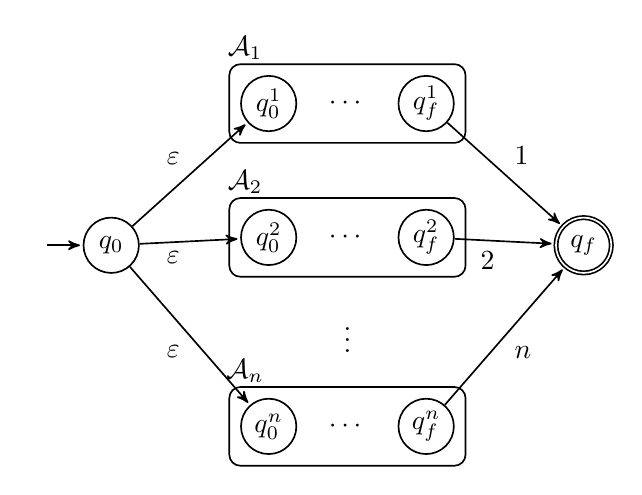
\begin{tikzpicture}[->, >=stealth', shorten >=1pt, auto, semithick, every state/.style={inner sep=0pt, minimum size=20pt}]
		\node[state, initial, initial text=] (0) at (0, 0) {$q_0$};
		
		\node at (1.7, 2.5) {$\mathcal{A}_1$};
		\draw[black, rounded corners] (1.5, 2.3) rectangle (4.5, 1.3);
		\node[state] (01) at (2, 1.8) {$q_0^1$};
		\node[state] (f1) at (4, 1.8) {$q_f^1$};
		\node (d1) at (3, 1.8) {$\cdots$};
		
		\node at (1.7, .8) {$\mathcal{A}_2$};
		\draw[black, rounded corners] (1.5, .6) rectangle (4.5, -.4);
		\node[state] (02) at (2, .1) {$q_0^2$};
		\node[state] (f2) at (4, .1) {$q_f^2$};
		\node (d2) at (3, .1) {$\cdots$};
		
		\node (dv) at (3, -1.1) {$\vdots$};		
		
		\node at (1.7, -1.6) {$\mathcal{A}_n$};
		\draw[black, rounded corners] (1.5, -1.8) rectangle (4.5, -2.8);
		\node[state] (0n) at (2, -2.3) {$q_0^n$};
		\node[state] (fn) at (4, -2.3) {$q_f^n$};
		\node (dn) at (3, -2.3) {$\cdots$};
		
		\node[state, accepting] (f) at (6, 0) {$q_f$};
		
		\path (0) edge node {$\varepsilon$} (01)
			(0) edge node[below left] {$\varepsilon$} (02)
			(0) edge node[below left] {$\varepsilon$} (0n)
			(f1) edge node {$1$} (f)
			(f2) edge node[below left] {$2$} (f)
			(fn) edge node[below right] {$n$} (f);	
	\end{tikzpicture}
	\caption{Skizze des NFAs aus Algorithmus~\ref{alg:algorithm}.}
	\label{fig:nfa}
\end{figure}
\end{document}